% The Why of Tali Forth
% Scot W. Stevenson

\section{The big picture}

This section provides background information on Forth, the 6502 processor, and
why anybody would want to combine the two. It can be safely skipped if you
already know all those things.

\subsection{The 6502 MPU}

Humanity reached the apex of processor design with the 6502\index{6502} in 1976.
Created by a team including Chuck Peddle\index{Peddle, Chuck} and Bill
Mensch\index{Mensch, Bill}, it was the engine that powered the 8-bit home
computer revolution of the 1980s.\footnote{Rumor has it that there was another
MPU called `Z80'\index{Z80} at the same time, but it ended up being a mere
footnote.} The VIC-20\index{VIC-20}, Commodore PET\index{Commodore PET}, Apple
II\index{Apple II}, and Atari 800\index{Atari 800} all used the 6502, among
others. 

\begin{figure}[h !]
        \centering
        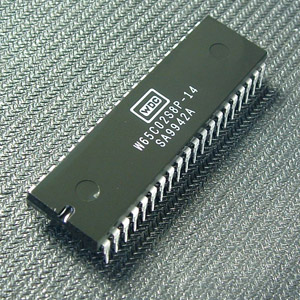
\includegraphics[width=0.5\textwidth]{pics/W65c02}
        \caption{\textit{The 65c02 MPU.} Photo: Anthony King, released in 
        the public domain}
        \label{fig:65c02}
\end{figure}

More than 40 years later, the processor is still in production by the \href
{http://www.westerndesigncenter.com/wdc/w65c02s-chip.cfm}{Western Design
Center}\index{WDC}. Apart for commercial uses, there is an active hobbyist scene
centered on the website \href{http://6502.org/}{6502.org}.\index{6502.org} Quite
a number of people have built their own 8-bit computers based on this chip --
there is even \href{http://wilsonminesco.com/6502primer/}{a primer} by Garth
Wilson\index{Wilson, Garth} to help you get started. It is for these systems
that Tali Forth 2 was created.

The most important variant of the 65c02 produced today is the \href
{https://en.wikipedia.org/wiki/WDC\_65C02}{65c02}\index{65c02}, a CMOS chip with
some additional instructions. Again, it is specifically for this chip that Tali
Forth 2 was written. 

But why program in 8-bit assembler at all?\footnote{Garth Wilson\index{Wilson,
Garth} answers this question in greater detail as part of his
\href{http://wilsonminesco.com/6502primer/65tutor\_intro.html}{6502 primer}} The
65c02 is fun to work with because of its clean instruction set architecture
(ISA)\index{instruction set!architecture}\index{ISA|see {instruction set}}. This
is not the place to explain the joys of assembler. The official handbook for the
65c02 is \textit{Programming the 65816, including the 6502, 65C02 and
65802}\cite{eyeslichty}.

\subsection{Forth}

\begin{quote}
        [I]f C gives you enough rope to hang yourself, Forth is a flamethrower
        crawling with cobras.
\end{quote}
\begin{flushright}
        -- Elliot Williams,\index{Williams, Elliot} \href{https://hackaday.com/2017/01/27/forth-the-hackers-language/}{
        \textit{Forth: The Hacker's Language}}
\end{flushright}

Forth\index{Forth|textbf} is the \textit{enfant terrible} of programming
languages. It was invented by Chuck Moore\index{Moore, Chuck} in the 1960s to do
work with radio astronomy before there were modern operating systems or
programming languages. A language for people who actually need to get things
done, lets you run with scissors, play with fire, and cut corners until you've
turned a square into a circle. Forth is not for the faint-hearted: It is
trivial, for instance, to redefine 1 as 2 and \texttt{true} as \texttt{false}.
However, Forth excels when you absolutely, positively have to get something done
with hardware that is actually too weak for the job. It rewards brilliance and
punishes stupidity.

It should be no surprise that NASA\index{NASA} is one of the organizations who
have made use of the language. The \textit{Cassini}
mission\index{Cassini@\textit{Cassini}} to Saturn used a
\href{http://www.cpushack.com/2013/02/21/charles-moore-forth-stack-processors/}{Forth
CPU}, for instance. It is also perfect for small computers like the 8-bit 65c02.
After a small boom in the 1980s, more powerful computers led to a decline in the
language. The `Internet of Things' with embedded small processors has led to a
certain amount
\href{https://www.embedded.com/design/programming-languages-and-tools/4431133/Go-Forth-}{renewed
interest} in the language. It helps that Forth is easy to implement: It is
stack-based, uses reverse polish notation (RPN)\index{RPN|see {reverse polish
notation}}\index{reverse polish notation} and a simple threaded interpreter
model. 

There is no way this document can provide an adiquate introduction to Forth.
There are quite a number of tutorils, however, such as \textit{A Beginner's
Guide to Forth} by J.V.~Nobel\cite{nobel} or the classic (but slightly dated)
\textit{Starting Forth}\cite{brodie03} by Leo Brodie\index{Brodie, Leo}.
Gforth,\index{Gforth} one of the more powerful free Forths, comes with its own
\href{http://www.complang.tuwien.ac.at/forth/gforth/Docs-html/Tutorial.html}{tutorial}.\footnote{Once
you have understood the basics of the language, do yourself a favor and read
\textit{Thinking in Forth} by Brodie\cite{brodie84}\index{Brodie, Leo}, which
deals with the philosophy of the language. Like Lisp\index{Lisp}, exposure to
Forth will change the way you think about programming.} 


\section{Writing your own Forth}

Even if the 65c02 is great and Forth is brilliant, why got to the effort of
writing a new, bare-metal programming language? Shouldn't there be a bunch of
Forths around already?


\subsection{FIG Forth}

In fact, the classic Forth availble for the whole group of 8-bit MPUs is FIG
Forth\index{FIG Forth}. There are PDFs of the
\href{http://www.forth.org/fig-forth/fig-forth\_6502.pdf}{6502 version} from
September 1980 freely available -- Forths are traditionally placed in the public
domain -- and more than one hobbyist has ported it to his machine. 

However, Forth has changed a lot in the past three decades. FIG Forth has been
replaced by the \href{https://forth-standard.org/}{ANSI Forth
standard}\index{ANSI Forth}, which includes such basic changes as how the
\texttt{do} loop works. Learning the language with FIG Forth is like learning
English with \textit{The Canterbury Tales}.\index{Canterbury Tales,
The@\textit{Canterbury Tales, The}}


\subsection{The need for a modern Forth for the 6502}

Tali Forth was created to provide an easy to understand modern Forth written
especially for the 65c02 that anybody can understand, adapt to their own use,
and actually work with. As part of that effort, the source code is heavily
commented -- and this document tries to explain the internals.


